\documentclass[./Report_main.tex]{subfiles}
\begin{comment}
If you want a box around your answer and that answer is an
equation then use \boxed{$$ equation $$} 

if you want to indent a block of text:
\begin{adjustwidth}{cm of right indent}{cm of left indent}
% paragraph to be indented
\end{adjustwidth}

if you just want one indent for one line 
use \indent per intended indent per line

A sections numbers automatically, so if the number of 
the problem is out of order it would be easier to 
just indent and bold the sections and subsections
and not use the \section{} kind of commands

\newpage makes a new page

$normal math mode$
$$Special math mode$$

to include an image use
\includegraphics{image_name}
image_name is the file name (.png) without the extension. The file
name cannot have any spaces or any periods other than the one before
the file extension.

To include a codeblock use
\begin{lstlisting}
ExampleCode(blah, blah)
{
	it does tabbing and everything;
	for (coloring of major languages like java){
		add the folloing to the \lstset tuple:
			language=<name_of_language>;
	}
}
\end{lstlisting}

\end{comment}


\begin{document}

%\tableofcontents

%\thispagestyle{empty}
%\newpage
% If you want to change how the subsubsection's are numbered
%\renewcommand{\thesubsection}{\thesection.\alph{subsection}.} 

%\setcounter{page}{0}
\chapter{Language Tutorial}
\section{Setup}
\subsection{install dependencies}
\begin{verbatim}
Download libuv from the following link: http://dist.libuv.org/dist/v1.11.0/
Follow the instructions to install:
 sudo apt-get install automake
 sudo apt-get install libtoolize
 ./autogen.sh
 ./configure
 make
 make check
 sudo make install
 echo "export LD_LIBRARY_PATH=\"/usr/local/lib\"" >> ~/.bashrc
 source ~/.bashrc
\end{verbatim}
\subsection{install ocaml}
\begin{verbatim}
add-apt-repository ppa:avsm/ppa
apt-get update
apt-get install ocaml ocaml-native-compilers camlp4-extra opam
\end{verbatim}
\subsection{make pipeline executable}
\begin{verbatim}
navigate to the src folder
enter command 'make'
\end{verbatim}
\subsection{run tests}
\begin{verbatim}
navigate to the src folder
enter command 'python testall.py'
\end{verbatim}
\subsection{Run files with the pipeline executable as follows:}
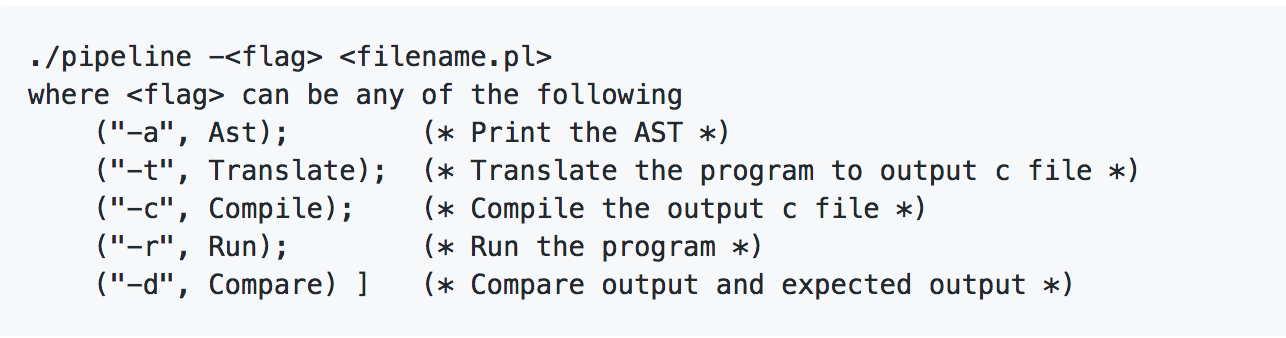
\includegraphics[scale = 0.5]{how_to_run}\\
\section{Program composition}
All statements in a pipeline program must be in one of the following blocks(function, pipe, anonymous block) with global variables as exception.\\
\begin{lstlisting}
    global int x = 10; // global variable not in a block, allowed
    
    
    
    function string hello(){
            return "hello" // statement in a function block, allowed
    }
    
    
    {
    int a;    //statements in anonymous block, allowed
    print_a
    }
    
    
    pipe{
        print_str("stmt in a pipe")// statement in a pipe block, allowed
    }
    
    
    print_int(x)// illegal, statement that's not in any block and not a global variable declaration.
\end{lstlisting}
\section{Variable declaration and assignment}
\subsection{primitive types}
pipeline has 4 primitive types:
\begin{itemize}
    \item int
    \item float
    \item string
    \item boolean
\end{itemize}
variable declaration for primitive types works as follow:
\begin{lstlisting}
    
int a; // type var-name for variable declaration
    
int b = 1;// type var-name expr, for variable declaration and initialization
    
a = 10; //variable assignment
\end{lstlisting}
\subsection{string manipulation}
String type supports the following operations:\\
\begin{itemize}
    \item len
    \item sub
    \item cmp
    \item concat(with \$)
\end{itemize}
\begin{lstlisting}
    string a = "hello";//declare string variable a
    
    string b = " world";//declare string variable b
    
    int length;
    
    length = len(a); // length = 5
    
    bool str;
    
    str = cmp(a,b);//str = false
    
    str = sub(a,b);//str = false
    
    string c = a$b;// c = "hello world" $
\end{lstlisting}
\subsection{global variables}
global variables in pipeline is declared with the \textbf{global} keyword and assessable throughout the program.\\
Also, global variable declaration need not to be inside a block.\\
\begin{lstlisting}
    global int a = 10;//global variable a.
    function int foo(){
            return a;//global variable a is accessible.
    }
\end{lstlisting}
\subsection{List}
List is a compound type that can be applied all primitive types. List cannot be declared globally like primitive types\\
The pipeline list is a singly likened list supports the the following operation:\\
\begin{itemize}
    \item addleft
    \item addright
    \item popleft
    \item list\_free
    \item access
\end{itemize}
\textbf{list-declaration}
\begin{lstlisting}[]
    int a[]; //int-list declaration
    
    float b[]; //float-list declaration
    
    string c[]; //string-list declaration
    
    bool d[]; //boo-list declaration
\end{lstlisting}
\textbf{list-append}
\begin{lstlisting}
    addleft(a,1) //append 1 to the left of a, a = [1]
    addright(a,2) // append 2 to the right of a, a = [1,2]
    popleft(a) // pop the left-most element in a, a = [2]
\end{lstlisting}
\textbf{list-access}
\begin{lstlisting}
    // let a = [1,2,3,4,5]
    a[0] //1
    a[1] //2
    a[4] //5
\end{lstlisting}
If a list is declared, it must be freed in order to prevent memory leak in the program
\textbf{list-free}
\begin{lstlisting}
    list_free(a)//release the memory of a and prevent memory leak
\end{lstlisting}
\subsection{struct}
Structs are a way for the user to define his/her own aggregate data type. It is a collection of variables that can be called and used for whatever purpose a user needs. \\
A struct must first be defined in the outermost scope before it can be used. It cannot be defined within a block, function or pipe. A struct can only contain a File, int, float, bool or string type, and only declarations without initialization may be used in the struct. The syntax to define a struct is with the \testtt{struct} keyword followed by the name of the struct and a block of statements between curly-braces and after the last curly brace there is a semicolon.
\begin{lstlisting}
/* struct definition */
struct struct_name {
     [declaration statements]
};
\end{lstlisting}
To use your struct in the body of your function simply use the \texttt{keyword} followed by the name of the variable. A struct variable must be declared in pipeline first, and it can never be initialized with a struct literal.
\begin{lstlisting}
/* proper struct declaration */
struct struct_name;
/* improper struct declaration */
struct struct_name = { [statements] };
\end{lstlisting}
the second case will fail compilation. In order to use the variables inside of the struct you simple use the struct variable name followed by dot operator "." and the name of the struct variable.
\begin{lstlisting}
/* struct use */
struct_name.variable = expr;
expr = struct_name.variable;
expr = expr + struct_name.variable; 
/* etc... */
\end{lstlisting}
Here is an example program that uses a struct:
\begin{lstlisting}
/* define the struct */
struct Example {
    int i;
    float f;
    bool b;
    string s;
    struct A a;
    File fl;
};
{
	struct Example e;
	e.s = "Hello World\n";
	e.i = 1;
	int i = e.1 + 1;
	if ( e.i < 3 ) {
	    print_string(e.s);
	}
}
\end{lstlisting}
\subsection{file}
File IO is done with a File object. First you must declare a File object and then use the init\_file\_obj function to initialize the file object and open the file. A file object cannot be initialized and declared in one statement.
\begin{lstlisting}
/* File declaration and initialization */
	File file_object;
	init_file_obj(file_object, file_name, file_mode);
\end{lstlisting}
for the init_file_obj you give it first the name of the file object, then a sting containing the name of the desired file, and lastly a string that represents the mode it can it is opened in. pipeline uses the standard c modes, so the mode must be one of the following strings:
\begin{lstlisting}
	mode	| mode description
	--------------------------------------------------------------------------------
	"r" 	| read-only mode
	"rb"	| read-only mode for a binary/unix style file
	"r+"	| read-mode but writing is also allowed
	"rb+"	| the same as "r+" but for binary/unix style files
	"w"		| write-only mode that creates a file or overwrites an existing file
	"wb"	| write-only but for binary/unix files
	"w+"	| write-mode that also allows reading
	"wb+"	| same as "w+" but for binary files
	"a"		| append-mode opens an existing file in write-only mode without overwriting the file
	"ab"	| same as "a" but for binary files
	"a+"	| append-mode with reading allowed
	"ab+"	| same as "a+" but for binary files
\end{lstlisting}
To write to a file you use the fwrite_str function, which takes a string and a file object as an argument, and then writes that string to a file.
\begin{lstlisting}
	fwrite_str(given_string, file_object);
\end{lstlisting}
To read a line from a file use the fread_line function which takes only the file object and returns a string. It reads up to the next newline character. To read up to 4095-bytes from a file in one chunk use the freadn function which takes a file object and an integer as an argument.
\begin{lstlisting}
	string s = fread_ln(file_object);
	s = freadn(file_object, number_of_bytes);
\end{lstlisting}
When you are done you must close the file to both prevent memory leaks and to ensure that the contents of the buffer are fully read into the file. To close a file object, use the function close_file which takes a file object as an argument and closes the file.
\begin{lstlisting}
	close_file(file_object);
\end{lstlisting}
In order to avoid memory leaks or file problems it is recomended that for write operations you open the file in either "w" or "a" mode write your strings and then 
close the file before you do any read operations, and for reading it is recommended to open in "r" or "rb" mode and do your read operations and then close the file before you do any write operations.\\
here is an example program:
\begin{lstlisting}
{
	File test_file;
	init_file_obj(test_file, "test-fileIO.txt", "w+");
	fwrite_str("Hello World\n", test_file);
	close_file(test_file);
	init_file_obj(test_file, "test-fileIO.txt", "r+");
	string s = fread_line(test_file);
	print_str(s);
	close_file(test_file);
	init_file_obj(test_file, "test-fileIO.txt", "r+");
	s = freadn(test_file, 4);
	print_str(s);
	print_str("\n");
	close_file(test_file);
}
\end{lstlisting}
\section{control flow}
control flow in pipeline works similar as C, it has for and wile loop and if, else selection\\
\begin{lstlisting}
{
    int a; 
    for(a = 0;a<10;a=a+1){// a for loop that loops over 10 times
        print_int(a);
    }
    a = 0;
    while(a<10){// a while loop that loops over 10 times
        print_int(a);
    }
    if(true){// an if selection that will always print false
        print_bool(false);
    }else{
        print_bool(true);
    }
}
\end{lstlisting}
The following program prints the lyrics for 99-bottles of beers.\\
\begin{lstlisting}
 {
 int i;
 for (i = 99; i >0; i = i-1)
     {
 
     string wall = " bottles of beer on the wall";
     string beer = " bottles of beer.";
     string pass = "Take one down and paas it around, ";
     string nomore = "No more bottle of beer on the wall";
     if(i>1){
         print_int(i);
         print_str(wall$", ");
         print_int(i);
         print_str(beer$"\n");
         print_str(pass);
         print_int(i-1);
         print_str(wall$".\n\n");
         }
     else{
         print_int(i);
         print_str(wall$",");
         print_int(i);
         print_str(beer$"\n");
         print_str(pass);
         print_str(nomore$"\n\n");
         print_str(nomore $ ", no more bottle of beer"$"\n");
         print_str("Go to the store and buy some more, 99 bottles of beer on the wall.\n");
         }
     }
     }
\end{lstlisting}
\section{function}
while pipeline has many buildin functions, it also allows custom function declaration. The fallowing function calculates the gcd of two given numbers and returns the result.\\
\begin{lstlisting}
function int gcd(int a, int b){
    while(a != b){
        if(a>b){
            a = a-b;
        }else{
            b = b-a;
        }
    }
    return a;
}
{
int result = gcd(14,21)// result = 7
}
\end{lstlisting}
pipeline also supports recursive functions.\\
\begin{lstlisting}
function int fib(int x){//function the calculates the nth Fibonacci numbers
 
     if(x==0){
         return 0;
     }
     if (x==1){
         return 1;
     }
     return fib(x-1)+fib(x-2);
 }
 {
 int c = fib(4);
 
 print_int(c);
 }
\end{lstlisting}
\section{pipe}
Pipes are created to enable asynchronous programming using the event-driven architecture. Ideally the code that is blocking, and the variables dependent on it, go inside a pipe. Multiple pipes can be created in the program.
\begin{lstlisting}
pipe{
	int a ;
	int b ;
	while(1);
	int c = a + b;
	print_int(a+b);
}
\end{lstlisting}

\section{Routing}
Pipeline language supports the following HTTP functions - LISTEN, GET, PUT, POST. All these functions are supported only inside a pipe. The Listen function has to go first inside the pipe before anything else, and the rest of the HTTP functions require LISTEN to be present for them to execute. The listen function takes a string (IP Address) and an integer (the port number). The other HTTP functions take “GET”, “POST”, “PUT”, “DELETE” as the 1st argument; the route as the 2nd argument; and the callback function(function name is passed as string) as the 3rd argument.

\begin{lstlisting}
function string get_user_handler(){
    return "You sent me a GET request !!!???! ";
}
function string put_user_handler(){
    return "You sent me a PUT request !!!???! ";
}
function string post_user_handler(){
    return "You sent me a POST request !!!???! ";
}
function string delete_user_handler(){
    return "You sent me a DELETE request !!!???! ";
}
pipe {
    listen("127.0.0.1",8080);
    http("GET","/user","get_user_handler");
    http("PUT","/user","put_user_handler");
    http("POST","/user","post_user_handler");
    http("DELETE","/user","delete_user_handler");
}

\end{lstlisting}
    


\section{build-in functions}
build-in functions provided by the pipeline language:\\
\begin{itemize}
    \item print\_int(int) - print a int to stdout
    \item print\_float(float) - print a float to stdout
    \item print\_bool(bool) - print a bool to stdout
    \item print\_string(string) - print a string to stdout
    \item print\_error(string) - print a string to stderr
    \item sleep(int) - block the program for a given number of seconds
    \item exit(int) - exit the program with given status
\end{itemize}
%\subsection{Identifiers}
%\subsubsection{}
%\subsection{subsection}
%\subsubsection{subsubsection}
\end{document}

